%%%%%%%%%%%%%%%%%%%%%%% file template.tex %%%%%%%%%%%%%%%%%%%%%%%%%
%
% This is a general template file for the LaTeX package SVJour3
% for Springer journals.          Springer Heidelberg 2010/09/16
%
% Copy it to a new file with a new name and use it as the basis
% for your article. Delete % signs as needed.
%
% This template includes a few options for different layouts and
% content for various journals. Please consult a previous issue of
% your journal as needed.
%
%%%%%%%%%%%%%%%%%%%%%%%%%%%%%%%%%%%%%%%%%%%%%%%%%%%%%%%%%%%%%%%%%%%
%
% First comes an example EPS file -- just ignore it and
% proceed on the \documentclass line
% your LaTeX will extract the file if required

%
%
%\documentclass{svjour3}                     % onecolumn (standard format)
%\documentclass[smallcondensed]{svjour3}     % onecolumn (ditto)
\documentclass{llncs}       % onecolumn (second format)
%\documentclass[twocolumn]{svjour3}          % twocolumn
%
%
\usepackage{graphicx}
%
% \usepackage{mathptmx}      % use Times fonts if available on your TeX system
%
% insert here the call for the packages your document requires
%\usepackage{latexsym}
% etc.
%
% please place your own definitions here and don't use \def but
% \newcommand{}{}
%
% Insert the name of "your journal" with
% \journalname{myjournal}
%
\begin{document}

\title{Automated Brain Disorders Diagnosis through Deep Neural Networks%\thanks{Grants or other notes
%about the artBrain Disorders Diagnosis Automation using Deep Neural Networksicle that should go on the front page should be
%placed here. General acknowledgments should be placed at the end of the article.}
}
%\subtitle{this is a  subtitle?\\ If so, write it here}

%\titlerunning{Short form of title}        % if too long for running head

\author{Gabriel A. Maggiotti (gmaggiotti@gmail.com)
\institute{Jampp.com}
}

%\authorrunning{Short form of author list} % if too long for running head


\date{Received: date / Accepted: date}
% The correct dates will be entered by the editor


\maketitle


\begin{abstract}
In most cases, the diagnosis of brain disorders such as epilepsy or a tumor is slow and requires endless visits to doctors and electroencephalogram (EEG) technicians. This project aims to automate brain disorder diagnosis by using Artificial Intelligence and deep learning. There are many brain disorders  can be detected by reading an Electroencephalography. Using an EEG device and collecting the electrical signals directly from the brain with a noninvasive procedure gives significant information about its health. Classifying and detecting anomalies on these signals is what doctors currently do when reading an Electroencephalography. With the right amount of data and the use of machine learning models, it could be possible to learn and classify these signals into groups like (i.e: anxiety, epilepsy spikes, abnormal tumor activity, etc). Subsequently, a trained Neural Network would interpret those signals and identify evidence of a disorder to automate the detection and classification of those disorders found. 
\end{abstract}


\paragraph{}\paragraph{}

\section{Introduction}
\label{intro}

This paper explores the use of a supervised machine learning approach to automate the detection of specific disorders on the brain by reading the EEG signals. Primarily, it focuses on Epilepsy and abnormal tumor activities.  Further research could extrapolate this approach to other brain conditions.

\paragraph{}
Epilepsy is a chronic disorder caused by an imbalance in the electrical activity of neurons in one or several areas of the brain. In most epilepsies, an anomaly in electrical activity can be observed through EEG by registering spikes in the affected areas.  These spikes have a unique pattern that can be seen with the naked eye on an electroencephalogram (spikes or peaks are registered with some frequency associated in the amplitudes of the electrical signals recorded).  Also tumors presents a unique pattern in the affected area that can be observed by an EEG.

\paragraph{}
These marks are indicators of the presence of the disorder. Patients carry this pattern of spikes almost all the time. Seizures or epileptic seizures are events of short duration, being the spikes the catalysts thereof.
\paragraph{}

\begin{figure}[h]
\centering
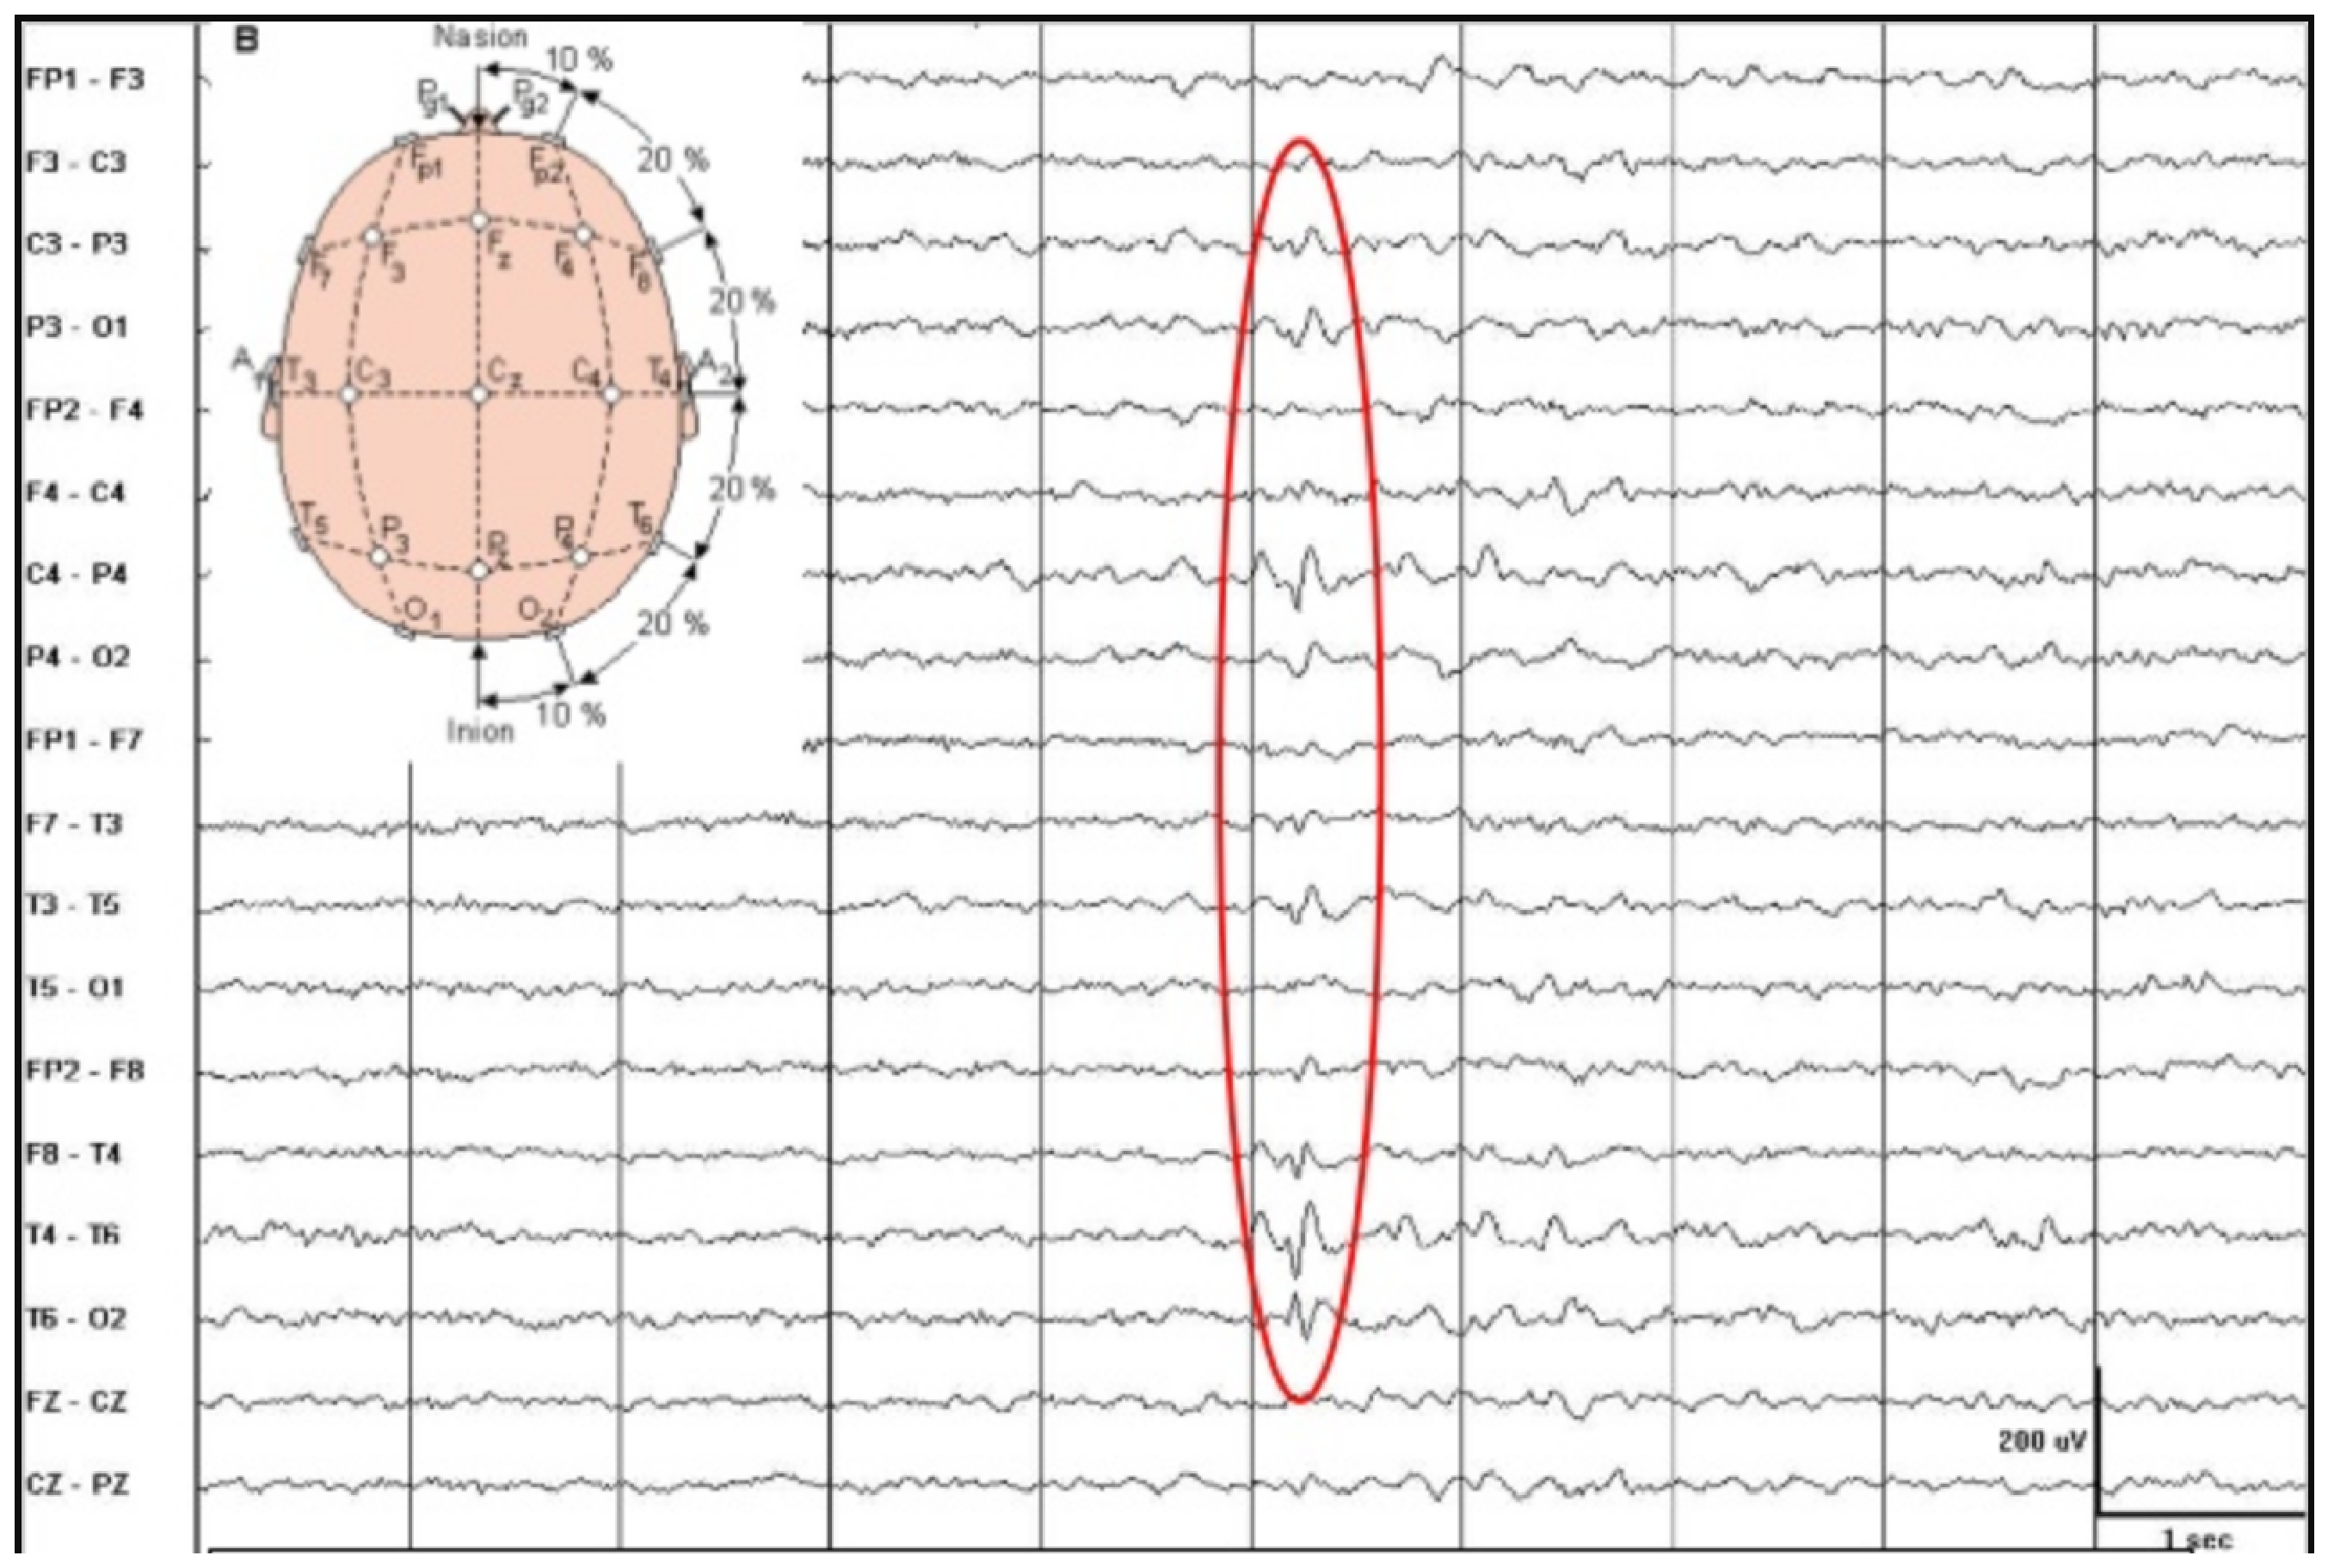
\includegraphics[width=6.08cm,height=4.36cm]{media/eeg-spike.eps}
\caption{Representative abnormal EEG waveforms.}
\end{figure}


This anomalous brain activity generates an observable mark or pattern. That footprint can be learned through a deep neural network. The following section will elaborate the whole process of data extraction and processing, as well as, the proposed five layers of fully connected Neural Network architecture for feature extraction. Furthermore, the process of training the network with a training-set followed by a validation of the results using a testing/validation set. 

\paragraph{}\paragraph{}

\section{References on the subject}
\label{sec:1}

In the past, there has been previous studies on epileptic seizure 
detection using pure EEG datasets. The following are the most relevant 
works on the subject (taken from $[$4$]$). The most common classifier 
used was support vector machine (SVM) and for dataset the CHB-MIT 
database. 


\paragraph{}
Related references using ANN with poor results $[$5$]$, $[$6$]$, 
$[$11$]$. No works found on the subject related with the use of deep neural networks.

\paragraph{}

Webber, 1996 $[$5$]$ ANN classification system SEN of 76\% and FPR of 1 event/h 

Pradhan, 1996 $[$6$]$  Wavelet transformation feature acquisition, ANN classification SEN of 97\% and SPEC of 89.5\% 

Gabor, 1998 $[$7$]$  Self-organizing neural network with unsupervised training SEN of 92.8\% and FPR of 1.35 events/h 

Wilson, 2004 $[$8$]$   matching pursuit,small neural networks, and clustering algorithm SEN of 76\% and FPR of 0.11 events/h 

Wilson, 2005 $[$9$]$  Used a trained probabilistic neural network SEN of 89\% and FPR of 0.56 events/h 

D'Alessandro, 2005 $[$10$]$  Genetic algorithm for signal processing, probabilistic neural network for classification 

Arabi, 2006 $[$11$]$  Used linear correlation feature selection methods and ANN. SEN of 91\% and FPR of 1.17 events/h 

Chan, 2008 $[$12$]$  SVM system SEN of 80-98\%, FPR of 38\% 

Netoff, 2009 $[$13$]$  Cost-sensitive SVM system SEN of 77.8\%, no false positives detected 

Chua, 2009 $[$14$]$  Data processing by higher-order spectra analysis and classification by the Gaussian mixture Acc=93\% 

Mirowski, 2009 $[$15$]$  Variable feature extraction methods used SEN71\% 
Sorensen, 2010 $[$16$]$  Features classified by matching pursuit algorithm and classified by SVM SEN of 78-100\% 

Chisci, 2010 $[$17$]$  Least-squares parameter estimator for extraction followed by SVM classification SEN of 100\% 

Peterson, 2011 $[$18$]$  Wavelet transform followed by SVM classification EEG SEN of 99.1\% and PPV of 94.8\% 

Temko, 2011 $[$19$]$  Fast Fourier transform used for feature extraction and SVM classification.  SEN 89\% 

Acharya, 2011 $[$20$]$  Higher-order spectra-based feature extraction followed by SVM, Detection accuracy of 98.5\% 

Kharbouch, 2011 $[$21$]$  Multistep feature extraction system followed by SVM classifier 97\% of seizures, FPR of 0.6 events/day 

Liu, 2012 $[$22$]$  Wavelet decomposition-based feature extraction  and by SVM  SEN of 94.5\% and SPEC of 95.3\% 

Direito, 2012 $[$23$]$  Markov modeling classification system. Identified four states - accuracy of 89.3\% 

Rabbi, 2012 $[$24$]$  Used fuzzy algorithms for feature extraction for classification SEN of 95.8\%


\paragraph{}
\section{Methodology: Dataset Processing}
\label{sec:2}

Dataset used was taken from The University of California Irvine [1].  UCI contains an Epileptic Seizure Data Set supported by 11500 measurements from a total of 500 individuals with each has 4097 data points for 23.5 seconds. Then divided and shuffled every 4097 data points into 23 chunks, each chunk contains 178 data points for 1 second, and each data point is the value of the EEG recording at a different point in time. So now we have 23 x 500 = 11500 pieces of information(rows), each information contains 178 data points for 1 second(columns), the last column represents the labels.  The dataset contains five different classes of 2300 samples each. Labels 1,2 and 5 were used respectively: class (1 for seizure activity; class (2 for abnormal tumor activity and class (5 for patients without seizures. Finally, two dataset were constructed.   For epileptic seizures samples of classes 1 and 5 were used (4600 samples).  And for tumor  activity classes 2 and 5 were used with the same number of samples.
   
\paragraph{}

To avoid saturation on the activation function and to make the gradient descent converge faster, the features were normalized to a range of values between -1 and 1 so that all features have a similar scale. The method used was standardization, which makes every feature have a zero mean value and unit variance. It is calculated for each feature as follows:


\begin{equation} 
x'=\frac{x-\hat{x}}{\sigma}
\end{equation}

\begin{equation}
\mu (x_{i})= 0   
\end{equation}

\begin{equation} 
\sigma (x_{i}) = \sigma(x_{j})
\end{equation}


\begin{figure}[h]
\centering
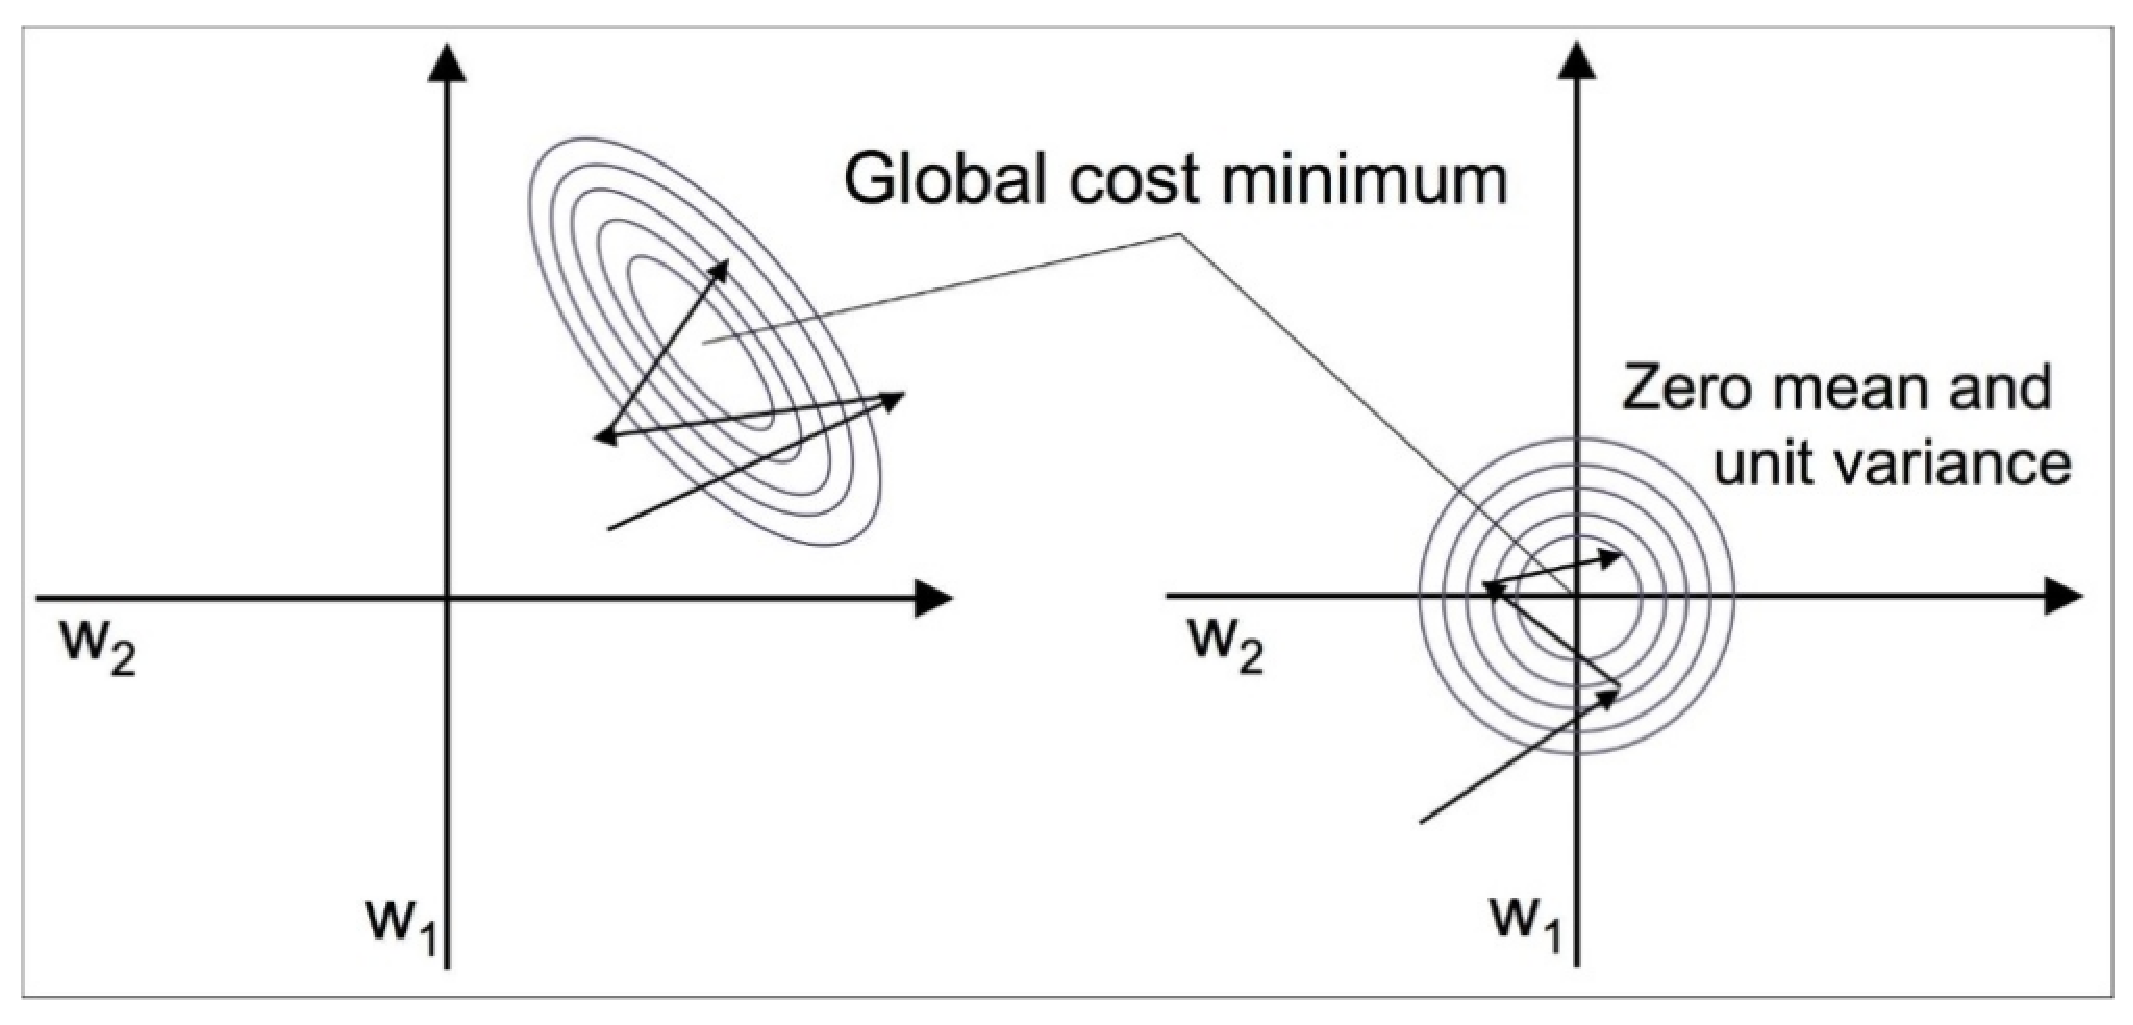
\includegraphics[width=9.81cm,height=5.00cm]{media/image7.eps}
\caption{Feature scaling is a method used to standardize the 
range of independent variables or features of data. In data processing, 
it is also known as data normalization and is generally performed during 
the data preprocessing step.}
\end{figure}

\paragraph{}
Lastly, the dataset will be further split into training, test and validation sets. It is very important that dataset is shuffled well to avoid any element of bias before training the ML model.

\paragraph{}

\section{Method / The Solution}
\label{sec:3}
Deep learning algorithms are composed of multiple processing layers that learn data representations with multiple levels of abstraction. Using a deep learning network (DNN) implemented in Python (TensorFlow library), we classified the subjects based on each label.  Design a fully connected Neural Network to capture the nonlinearity of the signals. 

The proposed architecture consists of five layers of fully connected neural networks (Fig. 3) to capture data nonlinearity. An Adam optimizer[50] was used because it is an efficient extension of stochastic gradient descent optimizers. The Adam optimizer achieves good results faster than other approaches and is used for objective function minimization by iteration. It computes individual adaptive learning rates from estimates of the first and second moments of the gradients.

\paragraph{}
Parameter initialization included assigning random values between 0 and 1 to the weights and zero values to the biases. However, for the dataset with all features and after feature selection, Xavier initialization was applied to the weights following Eq. 1 to obtain a global minimum of the cost function faster and more efficiently: 

\begin{equation} 
\theta\Rightarrow\theta=\{W_{0},W_{1},W_{2}...,W_{L}\}
\end{equation}

\begin{equation} 
Xavier = \sqrt{\frac{2}{features}}
\end{equation}

\paragraph{}
The weights were still random, but positive and negative values close to 0 were assigned to produce outputs that followed a similar distribution across all neurons. Supplementary Table 4 shows the initialization of the learning rates and the Xavier values for each dataset

\paragraph{}
The nonlinear sigmoid function was applied as the activation function of hidden layers. The objective function used measures the error between the neural networks output and the actual target, as shown in Eq. 7: 

\begin{figure}[h]
\centering
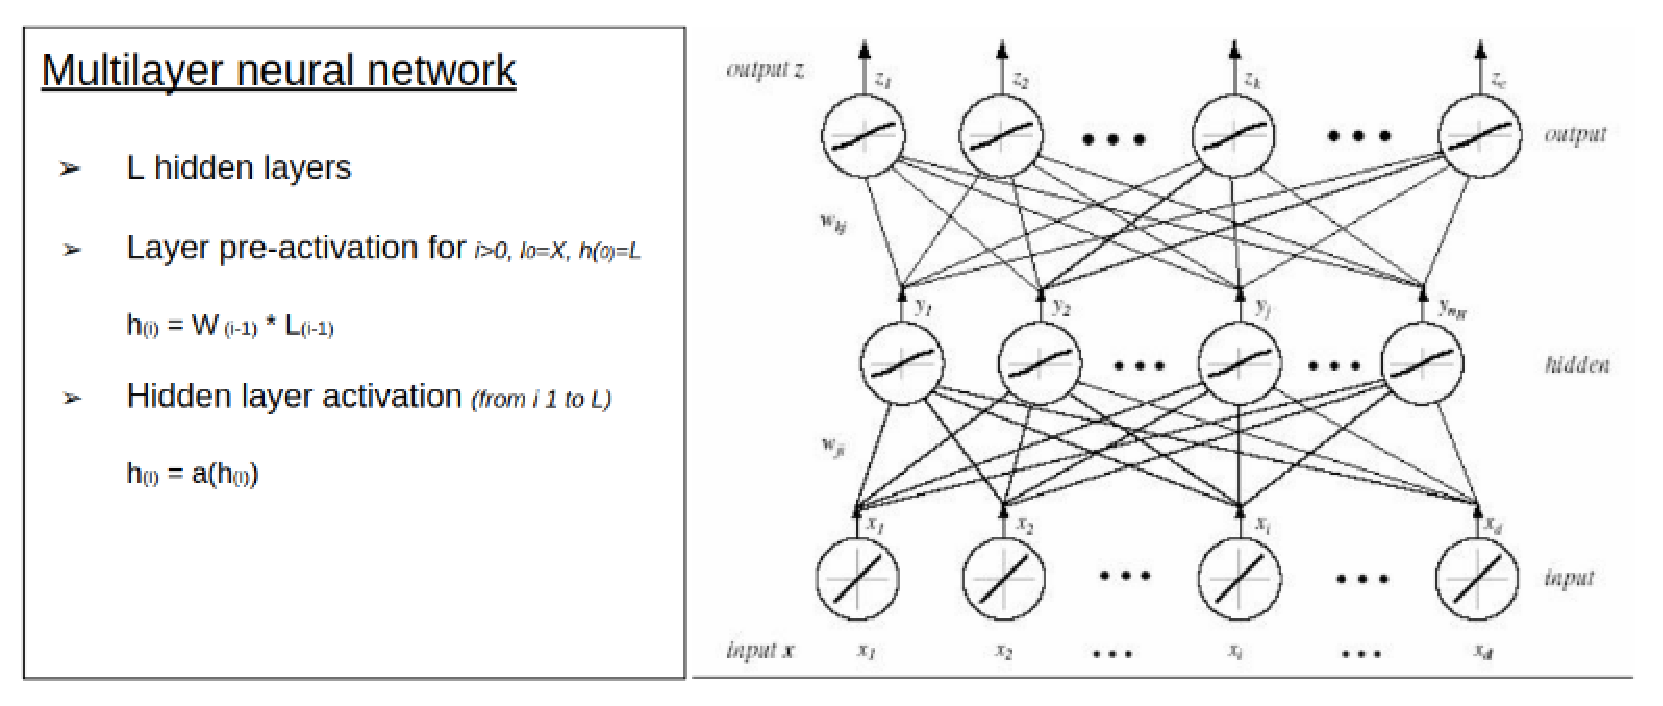
\includegraphics[width=10.51cm,height=4.77cm]{media/deep-nn.eps}
\caption{Architecture for a four layer fully connected 
Neural Network}
\end{figure}


\paragraph{}Iterate for N epochs,  for each training example Xi, Yi 
\begin{equation} 
g(x)^{i+1}=\sum_j^n(x_{j}*w_{j})\Rightarrow X^{i}*W^{i}
\end{equation}

\paragraph{}
Hidden activation layers are components that introduce non-linearity to 
the system. That Allows to capture and perform very sophisticated type 
of classification functions.
\begin{equation} 
L^{i+1}=sigmoid(g(x)^{i+1})
\end{equation}

\paragraph{}Calculate the error comparing the output of the NN with the actual target 
\begin{equation} 
Error = \frac{1}{2}\sum_i^n( y -\widehat{y})^2
\end{equation}

\begin{equation} 
\widehat{y}=Sigmoid(x_{i}\times w_{i})
\end{equation}

\paragraph{} Use the chain rule to efficiently compute gradients, top to bottom

\begin{equation} 
\frac{\partial E}{\partial w}=\frac{\partial }{\partial w} \frac{1}{2}\sum_i^n( y -\widehat{y})^2
\end{equation}

\begin{equation} 
\frac{\partial E}{\partial w} = \sum_i^n ( y -\widehat{y})  (-\frac{\partial E}{\partial w}\widehat{•}t{y})
\end{equation}

\begin{equation} 
\Rightarrow(\frac{\partial E}{\partial w}\widehat{y})= \widehat{y}(1-\widehat{y})
\end{equation}

\paragraph{}Back propagation of errors using the chain rule
\begin{equation} 
\nabla=\frac{\partial E}{\partial w}
\end{equation}

\begin{equation} 
\nabla_{n-1}=\nabla{n}*W^{T}_{n-1}
\end{equation}

\paragraph{}
As a regularization procedure for avoiding overfitting, a dropout approach was employed in the fourth hidden layers with a keep probability of 0.560. The optimization procedure was iterated until the minimum error on the training set and the maximum accuracy on the validation set (the number of observations that were correctly classified) were reached (Fig. 1ac and Supplementary Figure 4) and 5).
\paragraph{}

\paragraph{}\paragraph{}
\section{Results}
\label{sec:4}
Validation set, 1150 rows of information, was isolated from the the dataset.   The set was used to test the trained model, running it in each of the 1150 rows and comparing predictions with corresponded labels.  After 100 iterations, 99.96\% was reached.
\paragraph{}

\begin{figure}[h]
\centering
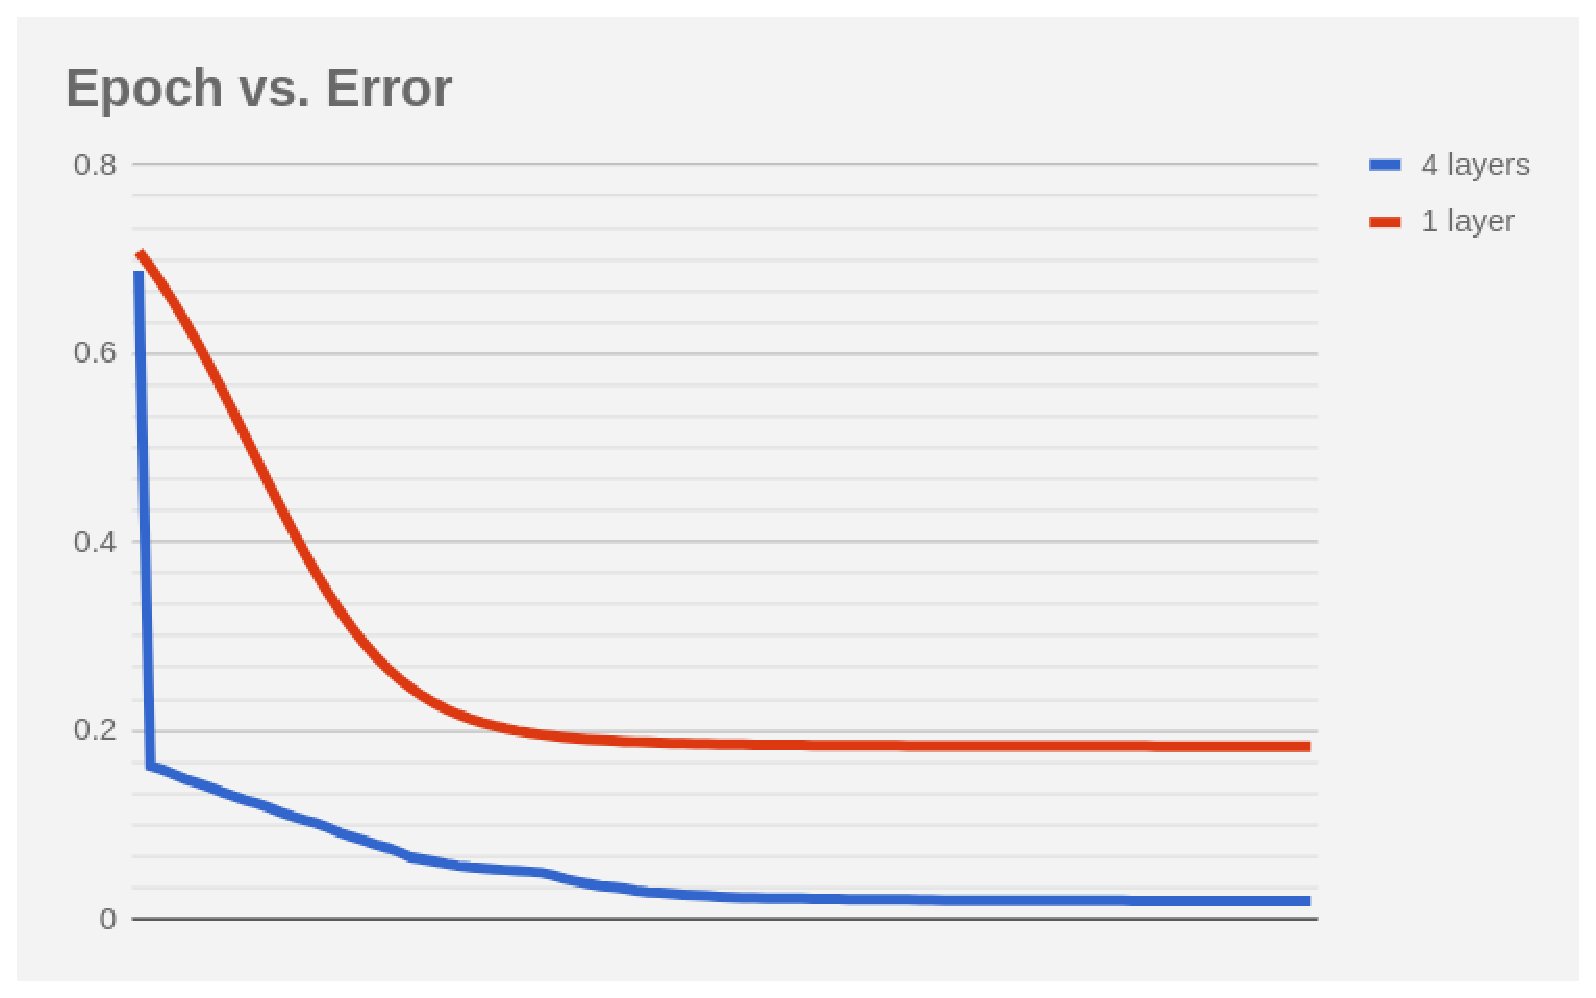
\includegraphics[width=9.08cm,height=5.11cm]{media/image10.eps}
\caption{ Error using 1 layer and 4 layers fully connected Neural Networks trained through 1000 epochs. 1 layer error:  0.175971;  4 layers error:  0.012657}
\end{figure}


\begin{figure}[h]
\centering
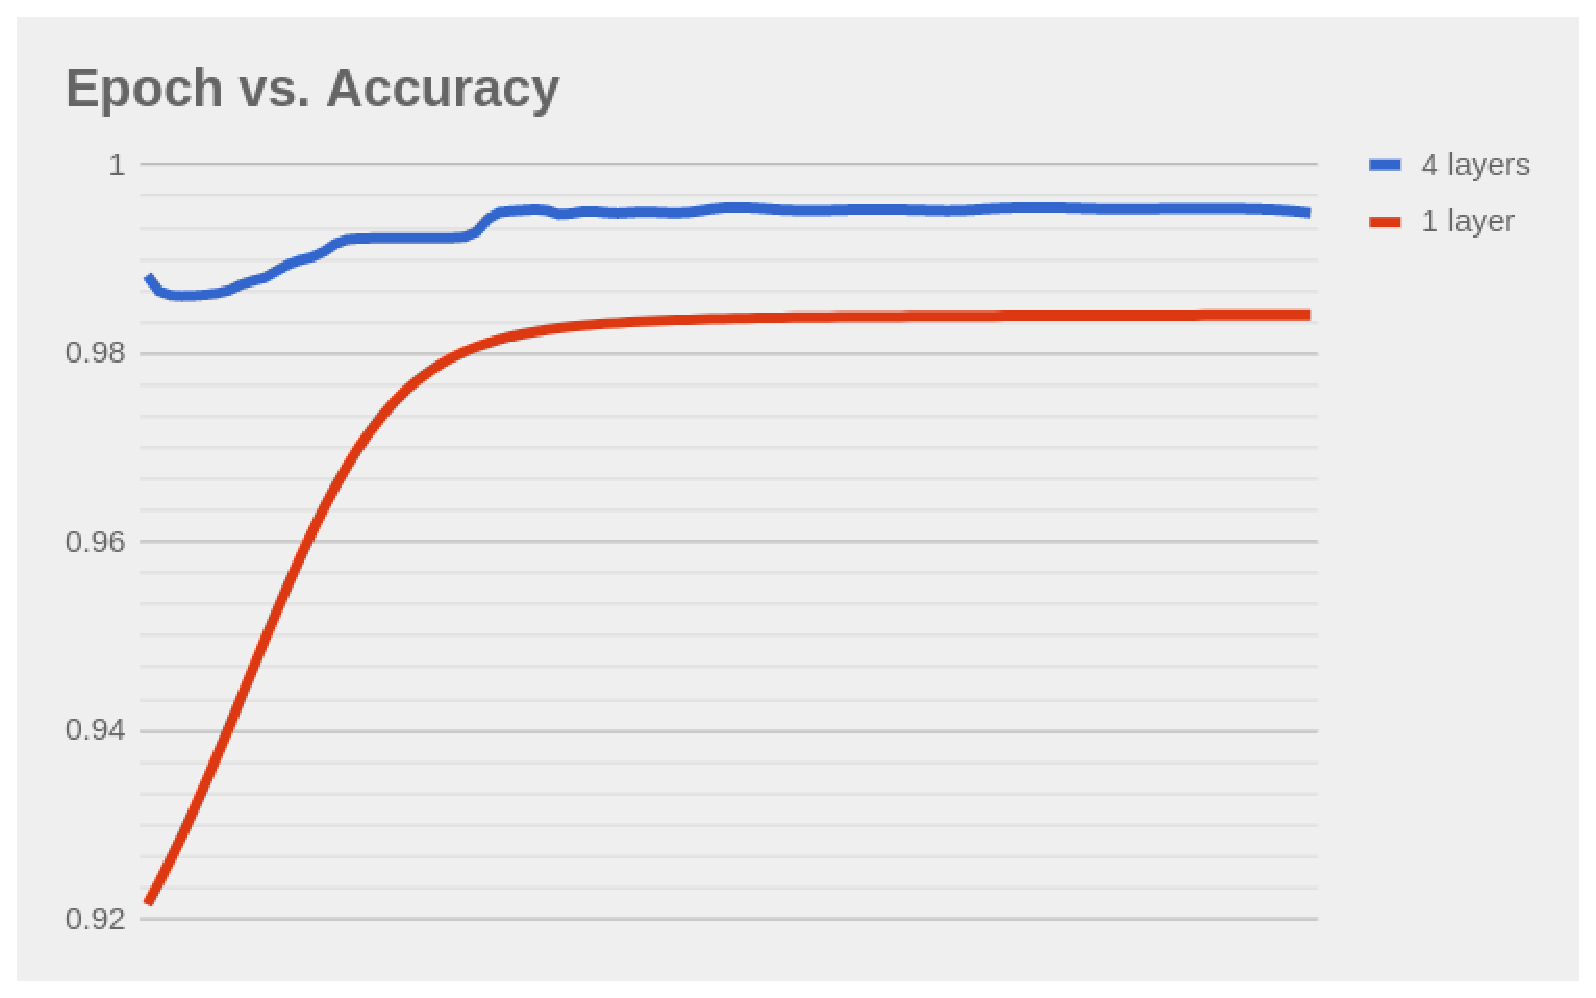
\includegraphics[width=9.00cm,height=5.07cm]{media/image11.eps}
\caption{Accuracy on test set using 1 layer and 4 layers fully 
connected Neural Networks trained through 1000 epochs. 1 layer accuracy: 
0.981064; 4 layers accuracy: 0.996806}
\end{figure}


\textbf{Hyper-parameters used: }learning rate 0.001, L2 Regularization with beta of 0.001, dropout with keep\_prob of \%50, Mini-batch / SGD 
- batch size 100; 1000 epochs; 11000 samples; 90\% for training set and 
10\% for validation set; improve of gradient descent through feature 
scaling; Sigmoid as activation function; also random weights and biases 
set to zero

 

\paragraph{}\paragraph{}

\section{Conclusion and Future Directions}
\label{sec:4}



 A successful automated detection and prediction of disorders introduces new innovative opportunities for diagnosis and preventive health care. This paper proposes a fast and lightway learning procedure for building a predictive model that satisfies the assignment. The use of deep neural networks in the subject turned out to be an excellent solution that presents high accuracy.  
\paragraph{}
The results are prominent and suggest that the model with existing clinical systems and practices may enable clinicians to make accurate epilepsy diagnosis and start  treatments earlier.
\paragraph{}
Moreover, it opens a door to extend the work on other areas like diagnosis of dementia, brain damage, brain diseases, psychiatric disorders, tumors, stroke, seizure forecasting from the study of interictal, preictal and ictal states and other focal brain disorders. 
\paragraph{}
Another area of interest would be Electrocardiogram signals. Further works can also be done on predicting heart attacks from ECG signals (people carrying holter monitors). 





% Non-BibTeX users please use
\begin{thebibliography}{}
%
% and use \bibitem to create references. Consult the Instructions
% for authors for reference list style.
%
\bibitem{RefJ}



$[$1$]$ - \underline{
https://archive.ics.uci.edu/ml/datasets/Epileptic+Seizure+Recognition}

$[$2$]$ - Andrzejak RG, Lehnertz K, Rieke C, Mormann F, David P, Elger 
CE (2001) Indications of nonlinear deterministic and finite dimensional 
structures in time series of brain electrical activity: Dependence on 
recording region and brain state, Phys. Rev. E, 64, 061907

$[$3$]$ - A.H. Shoeb, Application of Machine Learning to Epileptic 
Seizure Onset and Treatment, 2009.

$[$4$]$ - 
https://www.sciencedirect.com/science/article/pii/S1525505014002297

$[$5$]$ W.R. Webber, R.P. Lesser, R.T. Richardson, K. Wilson - An 
approach to seizure detection using an artificial neural network (ANN)

$[$6$]$ N. Pradhan, P.K. Sadasivan, G.R. Arunodaya - Detection of 
seizure activity in EEG by an artificial neural network: a preliminary 
study

$[$7$]$ A.J. Gabor -Seizure detection using a self-organizing neural 
network: validation and comparison with other detection strategies

$[$8$]$ S.B. Wilson, M.L. Scheuer, R.G. Emerson, A.J. Gabor - Seizure 
detection: evaluation of the Reveal algorithm

$[$9$]$ S.B. Wilson - A neural network method for automatic and 
incremental learning applied to patient-dependent seizure detection

$[$10$]$ M. D'Alessandro, G. Vachtsevanos, R. Esteller, J. Echauz, S. 
Cranstoun, G. Worrell, et al. - A multi-feature and multi-channel 
univariate selection process for seizure prediction

$[$11$]$ A. Aarabi, F. Wallois, R. Grebe - Automated neonatal seizure 
detection: a multistage classification system through feature selection 
based on relevance and redundancy analysis

$[$12$]$ A.M. Chan, F.T. Sun, E.H. Boto, B.M. Wingeier - Automated 
seizure onset detection for accurate onset time determination in 
intracranial EEG

$[$13$]$ T. Netoff, Y. Park, K. Parhi - Seizure prediction using 
cost-sensitive support vector machine

$[$14$]$ K.C. Chua, V. Chandran, U.R. Acharya, C.M. Lim - Automatic 
identification of epileptic electroencephalography signals using 
higher-order spectra

$[$15$]$ P. Mirowski, D. Madhavan, Y. Lecun, R. Kuzniecky - 
Classification of patterns of EEG synchronization for seizure prediction

$[$16$]$ T.L. Sorensen, U.L. Olsen, I. Conradsen, J. Henriksen, T.W. 
Kjaer, C.E. Thomsen, et al. - Automatic epileptic seizure onset 
detection using matching pursuit: a case study

$[$17$]$ L. Chisci, A. Mavino, G. Perferi, M. Sciandrone, C. Anile, G. 
Colicchio, et al. - Real-time epileptic seizure prediction using AR 
models and support vector machines

$[$18$]$ E.B. Petersen, J. Duun-Henriksen, A. Mazzaretto, T.W. Kjaer, 
C.E. Thomsen, H.B. Sorensen - Generic single-channel detection of 
absence seizures

$[$19$]$ A. Temko, E. Thomas, W. Marnane, G. Lightbody, G. Boylan - 
EEG-based neonatal seizure detection with Support Vector Machines

$[$20$]$ U.R. Acharya, S.V. Sree, J.S. Suri - Automatic detection of 
epileptic EEG signals using higher order cumulant features

$[$21$]$ A. Kharbouch, A. Shoeb, J. Guttag, S.S. Cash - An algorithm for 
seizure onset detection using intracranial EEG

$[$22$]$ Y. Liu, W. Zhou, Q. Yuan, S. Chen - Automatic seizure detection 
using wavelet transform and SVM in long-term intracranial EEG

$[$23$]$ B. Direito, C. Teixeira, B. Ribeiro, M. Castelo-Branco, F. 
Sales, A. Dourado - Modeling epileptic brain states using EEG spectral 
analysis and topographic mapping

$[$24$]$ A.F. Rabbi, R. Fazel-Rezai - A fuzzy logic system for seizure 
onset detection in intracranial EEG






\end{thebibliography}




\end{document}
